\chapter{Introdução}

\section{Enquadramento\label{se:enquadramento}}
Esta dissertação encontra-se no âmbito do projeto \href{https://traderes.eu/}{TradeRES}, que estuda um sistema de mercado elétrico capaz de atender às necessidades da sociedade num sistema quase totalmente renovável. Tendo as características para se integrar nos \href{https://ods.pt/ods/}{ \gls{ODS}} \ref{fig:ODS}. \\
O estudo da acessibilidade das energias renováveis ao mercado vigente integra-se nos \gls{ODS} n$^{\circ}$7, “Energia Renováveis e Acessíveis”, indo directamente de encontro a um dos pontos deste objectivo: 7.2.1 “Peso das energias renováveis no consumo total final de energia”. Por meio deste objectivo, a participação das renováveis no mercado faz também cumprir, embora indiretamente, o objectivo n$^{\circ}$8 “Trabalho Digno e Crescimento Económico”, através do ponto 8.4, onde é dada primazia à eficiência dos recursos globais no consumo e na produção. Indiretamente, pois, ao haver um melhor uso das renováveis, o uso de energias não limpas vai diminuir, melhorando a gestão de recursos, e baixando o consumo de recursos naturais não renováveis. \\
Por último podemos incluir o objectivo n$^{\circ}$13, “Acção Climática”, no qual, referimos de novo a diminuição de consumo de recursos finitos, mas mais importante, a melhor gestão de recursos renováveis. Promovendo o planeamento e estratégias de combate a emissões de gases de efeito estufa. \\

\begin{figure}[h]
    \centering
    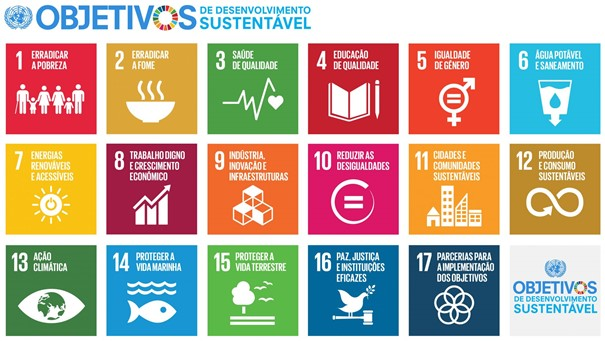
\includegraphics{Imagens/DesenvolvimentoSustentavel.jpg}
    \caption{Objectivos de Desenvolvimento Sustentável da ONU}
    \label{fig:ODS}
\end{figure}

\section{Objetivos e Perguntas de Pesquisa\label{se:objetivos}}

Foram aprovadas a nível europeu (2020) medidas de alteração aos serviços de sistema, que serão seguidas pelos Estados-Membros. Nesta dissertação, será realizada a aplicação dessas medidas, identificando as melhorias em relação ao design atual e avaliando se as novas medidas serão suficientes para garantir a operação de um sistema elétrico \textasciitilde100\% renovável, potencialmente identificando ações adicionais para garantir a robustez e segurança do sistema elétrico sem o uso de combustíveis fósseis. \\
A penetração das \gls{vRES} trouxe maior incerta na previsão e mercados de energia, pois estas estão mais sujeitos a elementos não controláveis como a velocidade do vento ou a radiação solar incidente.\\
As seguintes perguntas guiarão esta pesquisa.\\

\begin{enumerate}[label=\alph*)]
  \item Podemos reduzir a incerteza de grandes penetrações de \gls{vRES} na alocação de reserva secundária?
  \item A alocação dinâmica pode ter um efeito positivo no mercado de reservas?
  \item É possível prever a necessidade de reserva necessária baixando a alocação desperdiçada?
\end{enumerate}

Para responder a essas perguntas, utilizaremos dados de previsão de geração de energia renovável para estimar a energia necessária para alocação secundária. Atualmente, os valores de previsão desse mercado estão distantes do consumo real, o que resulta em alocações no dia anterior que não estão em conformidade com as necessidades reais. O objetivo deste trabalho é investigar se podemos obter previsões mais precisas da energia necessária utilizando técnicas de \textit{Machine Learning} (Aprendizado de Máquina). Isso possibilitará uma melhor gestão das alocações, resultando em um menor gasto de recursos energéticos e financeiros.

\section{Organização do Documento \label{se:organização}}

Este documento está dividido em capítulos. Sendo que os primeiros apresentam uma introdução às ideias e temas no \hyperref[ch:intro]{1}, o estado de arte dos temas na literatura publicada no \hyperref[ch:revisao]{2}, e por fim uma contextualização dos temas abordados no \hyperref[ch:contexto]{3}, contando também com o \hyperref[se:arch]{as arquiteturas} de modelos de machine learning utilizados nesta experiência.\\
Os dois capítulos seguintes apresentam os dois diferentes estudos. No \hyperref[ch:estudo_1]{capítulo 4} é definido e apresentado o resultado do estudo da estimativa do parâmetro $\rho$ da fórmula de estimativa da \gls{REN}.\\
No \hyperref[ch:estudo_2]{capítulo 5} explora-se o segundo estudo, o dimensionamento dinâmico da alocação necessária. São apresentados os dados utilizados com um estudo preliminar sobre os mesmos, e o tratamento necessário para usar nos modelos.\\
No \hyperref[ch:ferramentas]{capítulo 6} as ferramentas de programação criadas para realizar a mesma.\\
Os 3 capítulos seguintes são os descritivos da experiência em si. \hyperref[ch:metricas]{Capítulo 7} são as métricas usadas e criadas para a validação da experiência, \hyperref[ch:metodos]{capítulo 8} é a estrutura e parametrização da mesma, e \hyperref[ch:resultados_discussao]{capítulo 9} apresenta os resultados.\\
Termina com um \hyperref[ch:conclusao]{capítulo conclusivo} onde são avaliadas as experiências como um todo, e o seu impacto no âmbito dos mercados de reserva.\\